\documentclass[tikz,border=6pt]{standalone}
\usepackage[T1]{fontenc}
\usepackage{helvet}
\renewcommand{\familydefault}{\sfdefault}
\usetikzlibrary{positioning,arrows.meta,calc,fit,shapes.geometric,shapes.misc,shapes.multipart}
\newcommand{\dt}{\,\textperiodcentered\,}
\tikzset{
  arr/.style={-{Latex[length=2.2mm]},line width=0.6pt},
  darr/.style={{Latex[length=2.2mm]}-{Latex[length=2.2mm]},line width=0.6pt},
  dashedarr/.style={-{Latex[length=2.2mm,open]},line width=0.6pt,dashed},
  retarr/.style={-{Latex[length=2.2mm]},line width=0.6pt,dashed},
  lbl/.style={font=\footnotesize\itshape},
}

\tikzset{
  act/.style={draw,rounded corners=7pt,align=center,font=\small\bfseries,inner sep=7pt,minimum height=1.1cm,minimum width=3.6cm,line width=0.6pt},
  dec/.style={diamond,draw,aspect=2.2,align=center,font=\small\bfseries,inner sep=1pt,line width=0.6pt},
  start/.style={circle,fill=black,minimum size=6mm,inner sep=0pt},
  stop/.style={circle,draw,line width=1pt,minimum size=7mm,inner sep=0pt,path picture={\fill[black] (path picture bounding box.center) circle (2.2mm);}},
  bar/.style={fill=black,minimum height=1.4mm,inner sep=0pt},
  flow/.style={arr},
  g/.style={font=\footnotesize\itshape,fill=white,inner sep=1pt},
}

\begin{document}
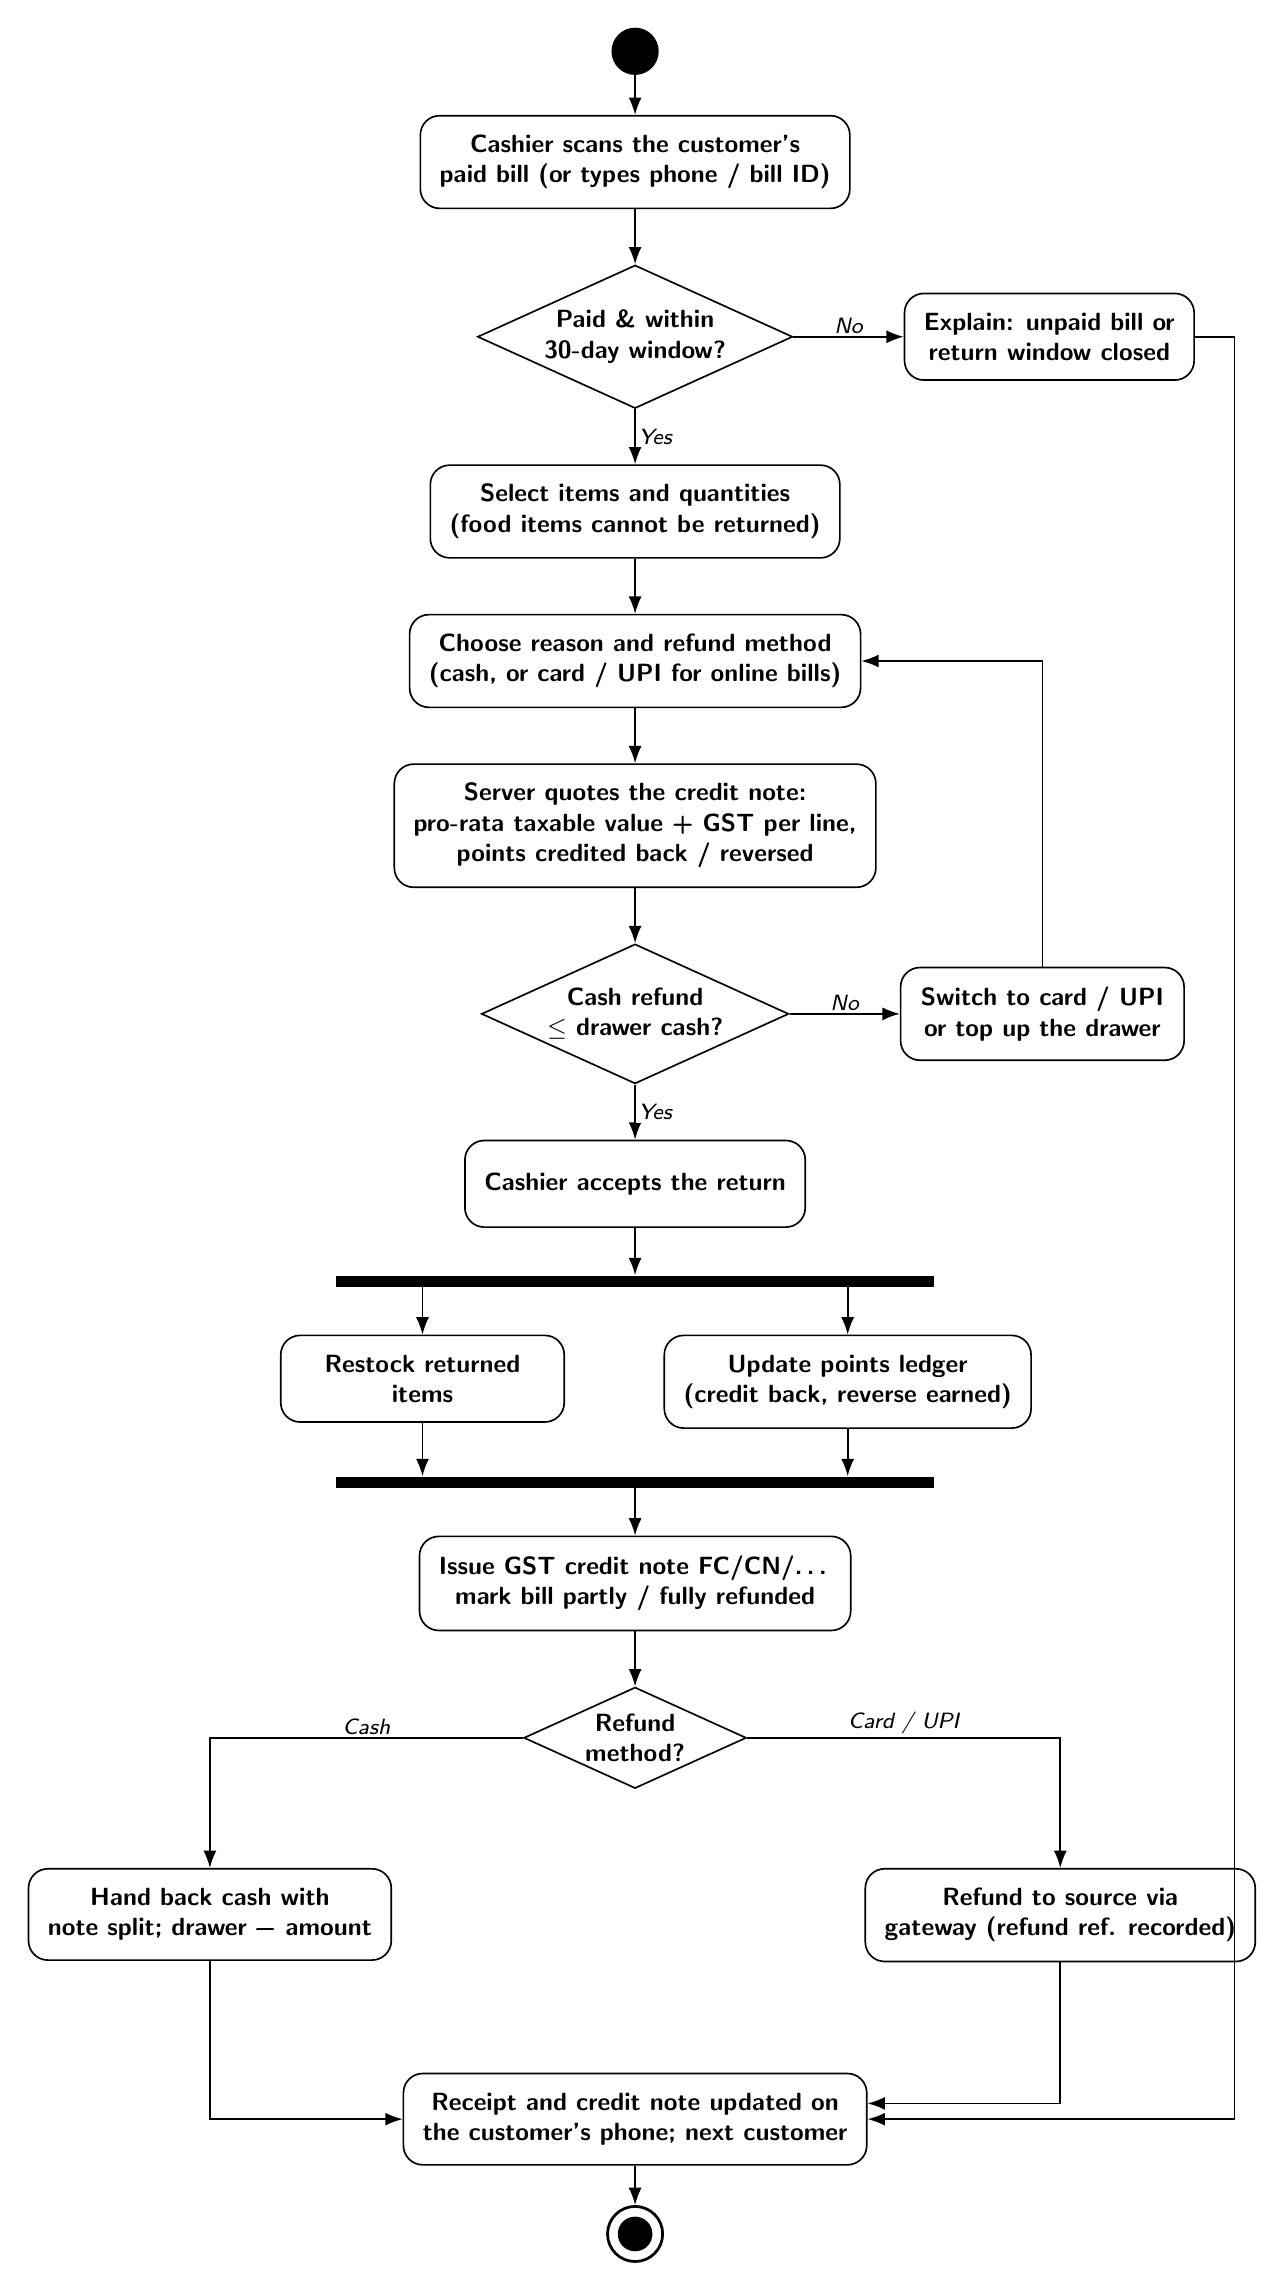
\begin{tikzpicture}[node distance=7mm and 12mm]
\node[start] (s) {};
\node[act,below=5mm of s] (a1) {Cashier scans the customer's\\paid bill (or types phone / bill ID)};
\node[dec,below=of a1] (d1) {Paid \& within\\30-day window?};
\node[act,right=14mm of d1] (no1) {Explain: unpaid bill or\\return window closed};
\node[act,below=of d1] (a2) {Select items and quantities\\(food items cannot be returned)};
\node[act,below=of a2] (a3) {Choose reason and refund method\\(cash, or card / UPI for online bills)};
\node[act,below=of a3] (a4) {Server quotes the credit note:\\pro-rata taxable value + GST per line,\\points credited back / reversed};
\node[dec,below=of a4] (d2) {Cash refund\\$\leq$ drawer cash?};
\node[act,right=14mm of d2] (no2) {Switch to card / UPI\\or top up the drawer};
\node[act,below=of d2] (a5) {Cashier accepts the return};
\node[bar,minimum width=7.6cm,below=6mm of a5] (fork) {};
\node[act,below=6mm of fork,xshift=-2.7cm] (p1) {Restock returned\\items};
\node[act,below=6mm of fork,xshift=2.7cm] (p2) {Update points ledger\\(credit back, reverse earned)};
\node[bar,minimum width=7.6cm,below=6mm of p2.south -| fork] (join) {};
\node[act,below=6mm of join] (a6) {Issue GST credit note FC/CN/\ldots\\mark bill partly / fully refunded};
\node[dec,below=of a6] (d3) {Refund\\method?};
\node[act,below=10mm of d3,xshift=-5.4cm] (r1) {Hand back cash with\\note split; drawer \textminus\ amount};
\node[act,below=10mm of d3,xshift=5.4cm] (r2) {Refund to source via\\gateway (refund ref. recorded)};
\node[act,below=36mm of d3] (a7) {Receipt and credit note updated on\\the customer's phone; next customer};
\node[stop,below=5mm of a7] (e) {};
\draw[flow] (s) -- (a1);
\draw[flow] (a1) -- (d1);
\draw[flow] (d1) -- node[g,above]{No} (no1);
\draw[flow] (no1.east) -- ++(0.5,0) |- (a7.east);
\draw[flow] (d1) -- node[g,right]{Yes} (a2);
\draw[flow] (a2) -- (a3);
\draw[flow] (a3) -- (a4);
\draw[flow] (a4) -- (d2);
\draw[flow] (d2) -- node[g,above]{No} (no2);
\draw[flow] (no2.north) |- (a3.east);
\draw[flow] (d2) -- node[g,right]{Yes} (a5);
\draw[flow] (a5) -- (fork);
\draw[flow] (fork.south -| p1) -- (p1);
\draw[flow] (fork.south -| p2) -- (p2);
\draw[flow] (p1) -- (p1 |- join.north);
\draw[flow] (p2) -- (p2 |- join.north);
\draw[flow] (join) -- (a6);
\draw[flow] (a6) -- (d3);
\draw[flow] (d3.west) -| node[g,above,pos=0.25]{Cash} (r1.north);
\draw[flow] (d3.east) -| node[g,above,pos=0.25]{Card / UPI} (r2.north);
\draw[flow] (r1.south) |- (a7.west);
\draw[flow] (r2.south) |- ($(a7.east)+(0,2mm)$);
\draw[flow] (a7) -- (e);
\end{tikzpicture}
\end{document}
